% !TeX spellcheck = pt_BR
% ------------------------------------------------------------------------
% ------------------------------------------------------------------------
% abnTeX2: Modelo de Trabalho Academico (tese de doutorado, dissertacao de
% mestrado e trabalhos monograficos em geral) em conformidade com 
% ABNT NBR 14724:2011: Informacao e documentacao - Trabalhos academicos -
% Apresentacao
% ------------------------------------------------------------------------
% ------------------------------------------------------------------------

\documentclass[
    % -- opções da classe memoir --
    12pt,               % tamanho da fonte
    openright,          % capítulos começam em pág ímpar (insere página vazia caso preciso)
    oneside,
    %twoside,           % para impressão em recto e verso. Oposto a oneside
    a4paper,            % tamanho do papel. 
    % -- opções da classe abntex2 --
    %chapter=TITLE,     % títulos de capítulos convertidos em letras maiúsculas
    %section=TITLE,     % títulos de seções convertidos em letras maiúsculas
    %subsection=TITLE,  % títulos de subseções convertidos em letras maiúsculas
    %subsubsection=TITLE,% títulos de subsubseções convertidos em letras maiúsculas
    % -- opções do pacote babel --
    english,            % idioma adicional para hifenização
    french,             % idioma adicional para hifenização
    spanish,            % idioma adicional para hifenização
    brazil              % o último idioma é o principal do documento
    ]{abntex2}

% ---
% Pacotes básicos 
% ---
\usepackage[utf8]{inputenc}
\usepackage{lmodern}            % Usa a fonte Latin Modern          
\usepackage[T1]{fontenc}        % Selecao de codigos de fonte.

\usepackage{lastpage}           % Usado pela Ficha catalográfica
\usepackage{indentfirst}        % Indenta o primeiro parágrafo de cada seção.
\usepackage{color}              % Controle das cores
\usepackage{graphicx}           % Inclusão de gráficos
\usepackage{microtype}          % para melhorias de justificação
\usepackage{longtable}          % para tabelas longas
\usepackage{tabularx,ragged2e}
\usepackage{multirow}
\usepackage{algpseudocode,algorithm}    % para algoritmos       
\usepackage{pdfpages}
\usepackage{subfig}
\usepackage{hyperref}
\usepackage{amsmath}
%\usepackage{subcaption}
% ---
        
% ---
% Pacotes adicionais, usados apenas no âmbito do Modelo Canônico do abnteX2
% ---
\usepackage{lipsum}             % para geração de dummy text
% ---

% ---
% Pacotes de citações
% ---
\usepackage[brazilian,hyperpageref]{backref}     % Paginas com as citações na bibl
\usepackage[alf]{abntex2cite}   % Citações padrão ABNT


%Espaçamento em formulas e tabelas
\renewcommand{\arraystretch}{1.3}
% --- 
% CONFIGURAÇÕES DE PACOTES
% --- 

% ---
% Configurações do pacote backref
% Usado sem a opção hyperpageref de backref
\renewcommand{\backrefpagesname}{Citado na(s) página(s):~}
% Texto padrão antes do número das páginas
\renewcommand{\backref}{}
% Define os textos da citação
\renewcommand*{\backrefalt}[4]{
    \ifcase #1 %
        Nenhuma citação no texto.%
    \or
        Citado na página #2.%
    \else
        Citado #1 vezes nas páginas #2.%
    \fi}%
% ---

% ---
% Informações de dados para CAPA e FOLHA DE ROSTO
% ---
\titulo{Avaliação do método do gradiente conjugado precondicionado para a solução paralela de um modelo de elementos finitos}
\autor{Thiago de Sousa Goveia}
\local{Timóteo}
\data{2017}
\orientador{Márcio Matias}
\instituicao{%
    Centro Federal de Educação Tecnológica de Minas Gerais
    \par
    Campus Timóteo
    \par
    Graduação em Engenharia de Computação
}
\tipotrabalho{Trabalho de conclusão de curso I (Graduação)}

% O preambulo deve conter o tipo do trabalho, o objetivo, 
% o nome da instituição e a área de concentração 
\preambulo{Proposta de trabalho apresentada como requisito das disciplinas trabalho de conclusão de curso I  e metodologia de pesquisa.}
% ---


% ---
% Configurações de aparência do PDF final

% alterando o aspecto da cor azul
\definecolor{blue}{RGB}{41,5,195}

% informações do PDF
\makeatletter
\hypersetup{
        %pagebackref=true,
        pdftitle={\@title}, 
        pdfauthor={\@author},
        pdfsubject={\imprimirpreambulo},
        pdfcreator={LaTeX with abnTeX2},
        pdfkeywords={abnt}{latex}{abntex}{abntex2}{trabalho acadêmico}, 
        colorlinks=true,            % false: boxed links; true: colored links
        linkcolor=blue,             % color of internal links
        citecolor=blue,             % color of links to bibliography
        filecolor=magenta,              % color of file links
        urlcolor=blue,
        bookmarksdepth=4
}
\makeatother
% --- 

% --- 
% Espaçamentos entre linhas e parágrafos 
% --- 

% O tamanho do parágrafo é dado por:
\setlength{\parindent}{1.3cm}

% Controle do espaçamento entre um parágrafo e outro:
\setlength{\parskip}{0.2cm}  % tente também \onelineskip

% ---
% compila o indice
% ---
\makeindex
% ---

% ----
% Início do documento
% ----
\begin{document}

% Seleciona o idioma do documento (conforme pacotes do babel)
%\selectlanguage{english}
\selectlanguage{brazil}

% Retira espaço extra obsoleto entre as frases.
\frenchspacing 

% ----------------------------------------------------------
% ELEMENTOS PRÉ-TEXTUAIS
% ----------------------------------------------------------
% \pretextual

% ---
% Capa
% ---
% \imprimircapa
% ---
% ---
% Folha de rosto
% (o * indica que haverá a ficha bibliográfica)
% ---
\imprimirfolhaderosto
% ---

% ---
% Inserir folha de aprovação
% ---

% Isto é um exemplo de Folha de aprovação, elemento obrigatório da NBR
% 14724/2011 (seção 4.2.1.3). Você pode utilizar este modelo até a aprovação
% do trabalho. Após isso, substitua todo o conteúdo deste arquivo por uma
% imagem da página assinada pela banca com o comando abaixo:
%
% \includepdf{folhadeaprovacao_final.pdf}
%
\iffalse
\begin{folhadeaprovacao}

  \begin{center}
    {\ABNTEXchapterfont\large\imprimirautor}

    \vspace*{\fill}\vspace*{\fill}
    \begin{center}
      \ABNTEXchapterfont\bfseries\Large\imprimirtitulo
    \end{center}
    \vspace*{\fill}
    
    \hspace{.45\textwidth}
    \begin{minipage}{.5\textwidth}
        \imprimirpreambulo
    \end{minipage}%
    \vspace*{\fill}
   \end{center}
        
   Trabalho aprovado. \imprimirlocal, 07 de abril de 2017:
   
   \assinatura{\textbf{Prof. \imprimirorientador} \\ Orientador} 
   \assinatura{\textbf{Prof. Marcelo de Sousa Balbino} \\ Coorientador}
   \assinatura{\textbf{Prof. Julio Cesar Onofre} \\ Professor Convidado}
   %\assinatura{\textbf{Professor} \\ Convidado 3}
   %\assinatura{\textbf{Professor} \\ Convidado 4}
      
   \begin{center}
    \vspace*{0.5cm}
    {\large\imprimirlocal}
    \par
    {\large\imprimirdata}
    \vspace*{1cm}
  \end{center}
  
\end{folhadeaprovacao}
\fi
%\includepdf{folhaaprovacao.pdf}
% ---

% ---
% Dedicatória
% ---
\iffalse
\begin{dedicatoria}
   \vspace*{\fill}
   \centering
   \noindent
   \textit{ Dedico esse trabalho à minha família, \\ fonte de motivação e educação.} \vspace*{\fill}
\end{dedicatoria}
\fi
% ---

% ---
% Agradecimentos
% ---
\iffalse
\begin{agradecimentos}
Agradecimentos...



\end{agradecimentos}
\fi
% ---

% ---
% Epígrafe
% ---
%\begin{epigrafe}
%    \vspace*{\fill}
%   \begin{flushright}
%       \textit{``Se os GAs são tão inteligentes,\\ por que eles não são ricos?''\\
%       (GOLDBERG, 1989, p.89)}
%   \end{flushright}
%\end{epigrafe}
% ---

% ---
% RESUMOS
% ---

% resumo em português
\setlength{\absparsep}{18pt} % ajusta o espaçamento dos parágrafos do resumo
\iffalse
\begin{resumo}
Resumo...

\textbf{Palavras-chave}: Palavras-chave...
\end{resumo}

% resumo em inglês
\begin{resumo}[Abstract]
 \begin{otherlanguage*}{english}
    Abstract...

   \vspace{\onelineskip}
 
   \noindent 
   \textbf{Keywords}: keywords...
 \end{otherlanguage*}
\end{resumo}
% ---

% ---
% inserir lista de ilustrações
% ---
\pdfbookmark[0]{\listfigurename}{lof}
\listoffigures*
\cleardoublepage
% ---

% ---
% inserir lista de tabelas
% ---
\pdfbookmark[0]{\listtablename}{lot}
\listoftables*
\cleardoublepage
% ---
\fi
% ---
% inserir o sumario
% ---
\pdfbookmark[0]{\contentsname}{toc}
\tableofcontents*
\cleardoublepage
% ---


% ----------------------------------------------------------
% ELEMENTOS TEXTUAIS
% ----------------------------------------------------------
\textual

% ----------------------------------------------------------
% Introdução (exemplo de capítulo sem numeração, mas presente no Sumário)
% ----------------------------------------------------------
\chapter{Contextualização}
	Devido à popularização da computação de alto desempenho (HPC), trabalhos recentes têm retomado problemas tradicionais a fim de adequá-los aos novos paradigmas e arquiteturas de computação. De acordo com \citeonline{Kiss2012} a conformidade entre o problema a ser resolvido e a estrutura do ambiente de execução é capaz de ampliar a performance e reduzir a energia dispendida no processamento.
	Devido ao aumento da demanda por recursos computacionais, dispositivos que possibilitam a execução paralela acabaram se estabelecendo no mercado da informática.
	Por meio das arquiteturas \textit{manycore} e \textit{multicore}, é possível se executar paralela ou concorrentemente tanto tarefas corriqueiras como a exibição de vídeos e jogos até cálculos complexos da ciência e da engenharia.
	Podem ser citados como processadores \textit{multicore} as linhas Core e Xeon da Intel\nocite{intel}, Opteron e Ryzen da AMD\nocite{amd} e a linha Power da IBM\nocite{ibm}. Os dispositivos manycore por sua vez, têm como principais representantes as unidades de processamento gráfico (GPU) da qual fazem parte as placas GeForce, Quadro e Tesla da NVIDIA\nocite{nvidia} e Radeon e FirePro da AMD\nocite{amd}.
	
	O método dos elementos finitos (FEM) é um método numérico para a resolução de problemas de valor de contorno (PVC) modelados por equações diferenciais e também de problemas associados à minimização de um funcional de energia \cite{Szabo2009}. O algoritmo clássico do FEM foi concebido em sua forma sequencial e consiste principalmente na solução de um sistema linear esparso. A tarefa de se resolver tal sistema é geralmente custosa em termos de memória quando adotados métodos diretos como a eliminação gaussiana e computacionalmente custosa quando adotados métodos iterativos como o método de Jacobi.
	O método dos gradientes conjugados (CG) e suas variantes pertencem à família dos métodos exatos/iterativos do subespaço de Krylov \cite{Anzt2016} e tem sido adotados na literatura para a solução paralela de elementos finitos. Alguns trabalhos correlatos que utilizam a família CG são apresentados por \citeonline{Yao2015}, \citeonline{Ahamed2016} e \citeonline{Iwashita2017}.
	
	A fim de adequar o FEM às arquiteturas modernas será adotado neste trabalho a abordagem elemento a elemento (EbE-FEM) proposta por \citeonline{Hughes1983}. Esta técnica baseia-se no fato de que a matriz do sistema de elementos finitos é caracterizada como uma função parcialmente separável \cite{Dayde1995}, resultado da soma das matrizes elementares. Assim sendo, as operações da solução do sistema de elementos finitos podem ser realizadas a nível elementar, sem a necessidade de se montar a matriz global do sistema. Adicionalmente tem-se a vantagem de que elementos não adjacentes podem ser calculados simultaneamente por meio dos métodos CG \cite{Wathen1989}. Esta última característica torna a técnica EbE-FEM propícia para a implementação paralela nas arquiteturas modernas.
	
	
	

	
\chapter{Problema}
	O problema \textit{benchmark} a ser modelado e resolvido como EbE-FEM refere-se à equação de Laplace originada do cálculo da distribuição de potencial e do campo elétrico de um capacitor de placas paralelas \cite[Exemplo 10.3]{boylestad2011}. 
	
	\section{Método Clássico}
	\subsection{Pré-processamento}
	
	A equação diferencial originada do PVC será resolvida em sua forma fraca, por meio da aproximação com polinômios lineares\cite{jin}. Em especial, será utilizado o método de Galerkin, cujas funções de base para os espaços de elementos finitos coincidem com as funções de aproximação \cite{jin}. Cada função de base é definida sobre o domínio de um elemento finito, o qual é obtido por meio da discretização  do domínio do problema. Para favorecer a precisão dos resultados a discretização será feita na forma de triangulação de Delaunay.	
	Após a geração do sistema de equações serão atribuídas a seus respectivos nós, as condições de contorno de Dirichlet prescritas no enunciado do problema. 
	
	\subsection{Processamento}
	O sistema de linear obtido na etapa de pré-processamento do método clássico será submetido ao solver do MATLAB\textsuperscript{\textregistered} e a algoritmos diretos e iterativos do framework implementado por \citeonline{Barrett1995} a fim de se realizar uma análise quantitativa dos métodos sequenciais. 
	
	\section{Método EbE}
	\subsection{Pré-processamento}
	O pré processamento do método EbE é similar ao do método clássico, exceto pelo fato de que a montagem do sistema global não é necessária. Adicionalmente, as condições de contorno também são atribuídas em nível elementar, utilizando-se um senso de média simples ou ponderada em cada nó, conforme apresentado nos trabalhos de \citeonline{Xu2005} e \citeonline{Yan2017} respectivamente. 
	
	\subsection{Processamento}
	O processamento elemento a elemento será realizado pelo método dos gradientes conjugados. Será feita uma análise comparativa do uso ou ausência de precondicionadores (Jacobi e Gauss-Seidel), conforme realizado no trabalho de \citeonline{Yan2017}.
	A implementação EbE será executada sequencialmente e também concorrentemente por meio e das linguagens C++11, Scala e Erlang, de forma similar ao trabalho de \citeonline{Boehmer2011}
	
	\section{Pós-processamento}
	Na etapa de pós-processamento os resultados de ambos os métodos serão coletados, tabulados e apresentados graficamente. As métricas gerais para uma análise quantitativa de desempenho serão o tempo de execução, consumo de memória e precisão dos resultados.
	Para o processamento paralelo também será utilizado o \textit{speedup} como métrica. 
	 Diferentes graus de refinamento da malha serão utilizados, de forma a verificar o limite de memória e e a relação entre o tempo de processamento e o número de nós.
	 
	\section{EbE em GPGPU}	
	 A segunda etapa deste trabalho (TCC II) tem como expectativa a implementação do EbE-FEM GPGPU (General Purpose Graphics Processing Unit) utilizando-se as mesmas métricas da programação \textit{multithreading}. Espera-se que seja possível a implementação nas linguagens CUDA (Compute Unified Device Architecture) e OpenCl(Open Computing Language) a fim de uma nova análise quantitativa, conforme apresentado no trabalho de \citeonline{Ahamed2016}.
	
\chapter{Justificativa}

A justificativa deste trabalho se baseia na contínua transformação dos paradigmas de programação e arquiteturas de hardware. Como coloca \citeonline{Guo2014}, com aumento de núcleos de processamento, ocorre a redução da razão memória por núcleo, o que impõe uma forte demanda para que os algoritmos utilizem eficientemente todos os níveis de paralelismo disponíveis enquanto minimizam a movimentação de dados. Tal evolução não se limita ao cenários dos \textit{clusters} e \textit{grids} mas alcança inclusive os dispositivos móveis, que atualmente já possuem até oito núcleos. Pensando em um futuro próximo, com os avanços da computação ubíqua que introduz temas como internet das coisas, dispositivos "usáveis", realidade aumentada e realidade virtual, a necessidade de se aproveitar ao máximo todo o poder de processamento disponível se torna ainda mais evidente, uma vez que nessas tecnologias há alta demanda de processamento e/ou pouco espaço físico para comportar um processador adequado. A justificativa para a escolha das linguagens C++11, Scala e Erlang se dá devido à ausência de trabalhos acadêmicos relacionando tais tecnologias e seu desempenho. C/C++ é uma linguagem abrangente, robusta e atual, presente por trás de grande parte das aplicações \textit{desktop} e \textit{mobile}. Scala e Erlang (e/ou Elixir \textit{bytecode}) são linguagens naturalmente concorrentes e que possuem crescente \textit{market share} \nocite{erlang}\nocite{scala}.


\chapter{Objetivos}

\section{Objetivos Gerais}

	\begin{itemize}
		\item Demonstrar o processo de mudança do paradigma sequencial para uma solução paralela do método do elementos finitos;
		\item Avaliar quantitativamente, segundo as métricas propostas (tempo de execução, uso de memória, precisão e \textit{speedup}) o desempenho das soluções de um modelo de elementos finitos;
		\item Apresentar à comunidade resultados acadêmicos experimentais do desempenho das  linguagens C++11, Scala e Erlang.
	\end{itemize}
		

\section{Objetivos Específicos}

	\begin{itemize}
		\item Investigar a viabilidade da técnica EbE-FEM como alternativa dos \textit{solvers} iterativos e do solver do  MATLAB\textsuperscript{\textregistered};
		\item Desenvolver um material acessível e de fácil compreensão de introdução ao FEM para o nível da graduação;
		\item Investigar o quão otimizada é a convergência do EbE a partir do emprego de diferentes precondicionadores;		
		\item Relacionar as métricas e conceitos de estatísticas necessários para a avaliação adequada de performance;
		\item Comparar conforme as métricas o desempenho das linguagens nativamente concorrentes na resolução do problema bechmark proposto neste trabalho.
	\end{itemize}

\chapter{Resultados Esperados}

Espera-se com este trabalho iniciar no CEFET-MG campus Timóteo uma nova linha de pesquisa a ser continuada nos trabalhos futuros, voltada para a análise numérica de problemas de valor de contorno da física aplicada. De forma similar, espera-se o incentivo e a adoção por parte da universidade de paradigmas e linguagens emergentes, de forma a diversificar o currículo dos graduandos.


\chapter{Cronograma}
	\begin{itemize}
		\item \textbf{27/07} - Entrega do texto do Referencial teórico e revisão bibliográfica;
		\item \textbf{31/07} - Entrega dos resultados preliminares;	
		\item \textbf{03/08} - Entrega do texto para a banca
		\item \textbf{17/08}  - Apresentação					
	\end{itemize}

\chapter{Estado da arte}
Como coloca \citeonline{Kiss2012}, o processamento paralelo de um problema modelado pelo FEM pode ser feito a partir da decomposição do domínio do problema. Esta decomposição pode ser feita por meio do particionamento da malha que representa o domínio do problema ou por meio da decomposição apropriada da matriz de coeficientes.
Os trabalhos de \citeonline{Boehmer2011} e \citeonline{Ahamed2016} apresentam a solução paralela do FEM por meio do particionamento da malha. No primeiro caso o processamento é executado comparativamente nas arquiteturas de memória compartilhada e distribuída com o uso da API OpenMP e da biblioteca MPI respectivamente.
No segundo caso, a comparação é feita entre as linguagens CUDA e OpenCL que são executadas em uma arquitetura \textit{manycore}. 

A técnica EbE é uma forma de decomposição da matriz de coeficientes e será tratada neste trabalho. Por meio desta, as operações são realizadas na matriz de cada elemento, sem que seja necessária a montagem do sistema global. Esta estrutura de dados foi proposta originalmente por \citeonline{Hughes1983} como uma fatoração especial para a matriz de coeficientes de forma a melhorar sua condição a acelerar a convergência \cite{Carey1988}. Devido ao seu desempenho, precisão, economia de memória e à possibilidade de processamento paralelo \cite{Levit1987, Jing2008, Kiss2012} a adoção da abordagem EbE tem sido recorrente à medida em que surgem novas tecnologias de HPC. 

\citeonline{Carey1988} apresenta uma implementação EbE do gradiente biconjugado (BiCG) para solucionar um sistema de elementos finitos (FE). Segundo ele, o surgimento de novas arquiteturas tais como os processadores vetoriais, paralelos e estações de trabalho microprocessadas foram responsáveis por se repensar o algoritmo original do FEM. A execução vetorial foi realizada no computador CRAY-XMP e foi $8$ vezes mais rápida em relação ao processamento sequencial e apresentou \textit{speed-up} variando de $4.25$ à $6.5$. A execução paralela foi feita no ALLIANT-FX/8, um mini supercomputador com $8$ CPUs. Foi adotado um esquema de ordenação de nós a fim de se evitar condições de corrida no acesso às variáveis globais. Com a utilização de todas as unidade de processamento, o \textit{speed-up} foi em torno de $7$ em relação ao uso de uma única CPU. 

O trabalho de \citeonline{Dayde1995} faz uma análise comparativa entre $5$ precondicionadores de nível elementar para o algoritmo do gradiente conjugado (CG), a saber: \textit{Element matrix factorization} (EMF), \textit{finite element preconditioner} (FEP), \textit{one-pass element-by-element preconditioner} (EbE), \textit{two-pass element-by-element preconditioner} (EbE2) e Gauss-Seidel \textit{element-by-element preconditioner} (GS-EBE). Como os autores colocam, uma vez que se têm problemas de larga escala mas parcialmente separáveis, torna-se necessário explorar diferentes alternativas a fim de se aproveitar as vantagens oferecidas pela estrutura do problema. A abordagem EbE se mostrou a melhor opção entre seus concorrentes. EMF e FEP requerem a montagem parcial do sistema, o que agrega maior custo de processamento. EBE2 e GS-EBE não apresentaram boas aproximações para elementos com pouca vizinhança. A fim de se realizar a paralelização, é sugerida a coloração da malha de forma que elementos vizinhos sejam processados sequencialmente.

Uma implementação EbE-CG em FPGA (Field Programmable Gate Array) é proposta por \citeonline{Jing2008}. Neste trabalho as operações sobre as matrizes elementares foram realizadas por meio da configuração de um circuito lógico no chip 4VLX160 da Xilinx. O processamento sequencial foi feito em um PC $2.01$ GHz Athlon $64$ com as devidas otimizações na compilação. Graças à implementação diretamente em hardware foi alcançado um \textit{speed-up} máximo igual a $40$.

O surgimento da linguagem CUDA em 2006 e a popularização das GPGPU possibilitaram que a técnica de EbE pudesse ser revisitada e aplicada nas arquiteturas modernas. \citeonline{Kiss2012} soluciona o um modelo de elementos finitos por meio do BiCG com precondicionador de Jacobi.  De acordo com este trabalho, a abordagem EbE é adequada para o processamento em GPU, cuja arquitetura embora seja massivamente paralela, possui um gargalo, que é a  capacidade limitada de memória. O caráter localizado do EbE faz com que o trânsito de dados seja mínimo, o que reduz o consumo de energia e maximiza o potencial do dispositivo. Para a realização dos testes foram utilizados o processador quad-core Xeon X3440 da Intel e a placa GTX 590 da NVIDIA, contendo $2$ GPUs. A execução com aceleração em GPU consumiu 20 vezes menos memória e foi 10 vezes mais rápida que a execução unicamente em CPU.

O trabalho de \citeonline{Wu2015} também apresenta o método BiCG elemento a elemento com precondicionador de Jacobi implementado em GPU. Foi utilizado o processador Xeon E5-2696v2 da Intel e a placa Tesla K20c da NVIDIA. Nos dois refinamentos de malha testados foi alcançado um \textit{speed-up} de $4.63$, e como coloca o autor, o resultado obtido se torna ainda mais efetivo à medida em que o número de elementos aumenta. No trabalho mais recente dos mesmos autores \cite{Yan2017} é apresentado o uso do precondicionador de Gauss-Seidel para a abordagem EbE, o qual apresentou melhores resultados para o número de iterações e tempo de execução em relação ao precondicionamento de Jacobi, mantendo a mesma precisão.

Outros trabalhos importantes para esta monografia são os de \citeonline{Xu2005}, \citeonline{Yao2015} e \citeonline{Chou2016}. O primeiro apresenta a implementação do EbE-CG e a técnica de atribuição das condições de contorno que também será empregada no presente trabalho. O segundo apresenta a comparação da performance da implementação do BiCG estabilizado (BiCGStab) em CPU e GPU, utilizando-se diferentes formas de armazenamento de matriz esparsa e diferentes ferramentas de resolução de sistema linear em GPU, a saber: CUSPARSE, CUSP e CULA Sparse. O último trabalho apresenta a comparação entre diferentes tecnologias de processamento paralelo (Cuda C, Cuda Fortran, MPI e OpenMP) na resolução de dois problemas \textit{benchmark}


\chapter{Fundamentação teórica}
% ---
Neste capítulo é apresentado o referencial teórico para a compreensão dos métodos e conceitos utilizados ao longo deste trabalho. 
Na \hyperref[sec:PVC]{primeira seção} é apresentada a definição de Problemas de Valor de Contorno (PVC) bem como o problema a ser solucionado neste trabalho. 
Na \hyperref[sec:SED]{seção seguinte}, são abordados os Sistemas de Elementos Discretos a fim de fornecer a compreensão intuitiva e genérica do Método dos Elementos Finitos.
Em seguida, na seção \ref{sec:FEM} é feita a introdução ao Método dos Elementos Finitos (FEM). 
As seções \ref{sec:preProc}, \ref{sec:proc} e \ref{sec:posProc} abordam respectivamente, as etapas de pré-processamento, análise e pós-processamento do FEM.
Nas seção \ref{sec:eletromag} são apresentadas as equações de Maxwell para o Eletromagnetismo e na seção \ref{sec:tecItera} são mostradas algumas técnicas iterativas para a resolução de sistemas lineares, tais como o Método do Gradiente Conjugado e o uso de Precondicionadores. Estas técnicas são as estratégias utilizadas para a realização da abordagem Elemento a Elemento (EbE) do FEM.
Por fim, a \hyperref[sec:GPGPU]{última seção} deste capítulo apresenta os principais fundamentos da programação de Uso Geral em Unidades de Processamento Gráfico (GPGPU).

\section{Problema de Valor de Contorno}
\label{sec:PVC}


Um problema de valor inicial \textbf{PVI},pode ser definido como uma equação ou sistema de equações diferenciais no qual são dadas as condições iniciais do fenômeno. Tais condições são impostas sobre a variável dependente e suas derivadas em um único instante de tempo (inicial) $t_0$. Um problema de valor de contorno \textbf{PVC} por sua vez, apresenta tais condições impostas em pontos distintos, como por exemplo em $x_i$ e $x_f$. Geralmente os PVI são dados em função do tempo enquanto os PVC são dados em função do espaço \cite{boyceDiprima}.

Como pode ser visto na tabela \ref{tab:cond}. as condições estabelecidas sobre a variável dependente, são chamadas de \textbf{condições de Dirichlet} ou \textbf{essenciais}, enquanto as que são estabelecidas sobre as derivadas da variável dependente são  conhecidas como \textbf{condições de Neumann} ou  \textbf{naturais}. Além destas duas, existem as restrições específicas do fenômeno modelado, como por exemplo, condições de radiação ou de impedância para problemas do eletromagnetismo \cite{jin}. 


\begin{table}   
	\centering
	\begin{tabular}{|c|c|}  
		\hline
		\textbf{Condição} 
		& \textbf{Tipo} \\  
		\hline
		$u(x_i) = \alpha $ 
		& Dirichlet \\
		\hline
		$u(x_i) = 0$
		& Dirichlet Homogênea\  \\
		\hline
		$u'(x_i) = \beta$
		& Neumann \\
		\hline
		$u'(x_i) = 0$
		& Neumann Homogênea\  \\
		\hline
	\end{tabular}
	\caption{Exemplos de condições de contorno}
	\label{tab:cond}
\end{table}


A solução analítica de um PVC pode ser obtida por meio da integração direta ou a partir da aplicação de técnicas como a separação de variáveis, expansão em séries ou pela transformada de Laplace.
No entanto, a maioria dos problemas da engenharia e da ciência não são lineares e apresentam geometria ou condições de contorno complexas.  Estas características fazem com que a resolução analítica de tais problemas seja impraticável, sendo necessário recorrer a métodos numéricos para se obter uma solução aproximada \cite{boyceDiprima, powers}.



\section{Métodos numéricos para PVCs}
\label{sec:FEM}

O método dos elementos finitos (FEM) é uma alternativa numérica para a solução de PVCs.Neste método, o domínio do problema é visto como uma coleção de subdomínios, chamados de elementos finitos, sobre os quais, a equação que modela o problema é aproximada por um método variacional ou de resíduos ponderados \citeonline{reddy}. Essas diferentes vertentes do método surgiram graças aos esforços independentes de matemáticos, cientistas e engenheiros \cite{zien}. 

O método das diferenças finitas (FDM) assim como o FEM é uma abordagem numérica para a aproximação de PVCs. Este método consiste na discretização do domínio do problema por meio de uma grade de pontos e na aproximação de cada derivada da equação por um quociente-diferença adequado
\cite{burdenFaires}. Embora este método seja útil em muitos casos, se torna difícil aplicá-lo em problemas com geometria irregular ou com condições de contorno não usuais.

Diferentemente do FDM, como coloca \citeonline{huebner}, o FEM divide o domínio não em pontos, mas em subdomínios, sobre os quais as equações são aproximadas por polinômios definidos por partes. O FEM também é capaz de representar mais fielmente o contorno (ou a borda) do problema. Desta forma, ele se apresenta como uma técnica mais poderosa e versátil para a modelagem de fenômenos com geometria complexa e meios não homogêneos \cite{sadiku}. 

\begin{figure}[!htb]
	\centering
	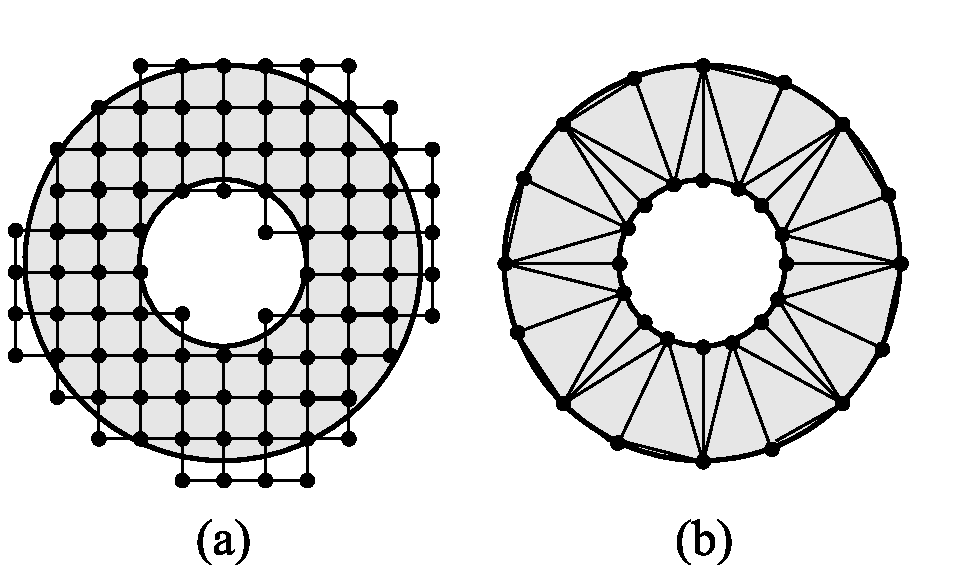
\includegraphics[scale=0.5]{figuras/fdm_fem.pdf}
	\caption{a)Método das diferenças Finitas b) método dos Elementos Finitos}
	\label{fig:mdfFem}
\end{figure}

\section{Método dos Elementos Finitos}

O FEM surgiu originalmente como uma técnica de análise de deslocamentos e elasticidade de estruturas mecânicas, mas em seguida foi estendido para solucionar problemas de outros campos da física e da engenharia \cite{jin, desai, zien}.

As primeiras formulações do FEM são conhecidas como \textbf{abordagem direta} ou \textbf{formulação física}, que embora forneça a interpretação intuitiva do método, é util apenas para a resolução de problemas relativamente simples \cite{huebner, desai, zien}. O uso do princípio do trabalho virtual, para a determinação de forças na abordagem direta, levou à generalização do FEM, por meio da estratégia de minimização do funcional de energia. Esta técnica mais genérica  ficou conhecida como \textbf{formulação variacional} \cite{desai, zien, jin} e tem como principal representante o método de Rayleigh-Ritz. Uma terceira abordagem, conhecida como \textbf{Método dos Resíduos Ponderados} ou \textbf{formulação generalizada} \cite{zien, huebner} é tradicionalmente utilizada e é ainda mais genérica que o princípio variacional, pois resolve diretamente as equações diferenciais do modelo, sem necessitar da existência de um funcional de energia \cite{desai}, ou ainda, sem exigir que o sistema seja positivo-definido. Neste trabalho será adotado o método dos resíduos ponderados, mais especificamente, o método de Galerkin.


\section{Método dos Resíduos Ponderados}
\label{sec:proc}

De acordo com \citeonline{jin}, a aplicação do FEM pode ser feita a partir de $4$ passos básicos, os quais serão detalhados nas subseções a seguir.


\subsection{Discretização do Domínio} 
A discretização do domínio consiste na transformação do contínuo $\Omega$ em uma malha de elementos finitos (discretos). Cada elemento $\Omega_e$ dessa malha representa um subdomínio de $\Omega$.  
Nesta etapa são definidas a forma, a quantidade e o tamanho dos elementos, de forma que a representação em malha seja a mais próxima possível do objeto em análise \cite{desai}.

Conforme pode ser visto na figura \ref{fig:numeracao}, cada elemento é identificado na malha a partir de um número que lhe é atribuído. Os vértices (ou nós) de cada elemento também são numerados. Cada nó possui dois valores vinculados a ele, um atuando como identificador global (numeração do nó na malha) e o outro como identificador local (numeração dentro de um dado elemento). A numeração local é geralmente feita no sentido anti-horário, a fim de se obter um valor positivo no cálculo da área ou volume por meio do  determinante \cite{sadiku, jin}. 

Um fator que deve ser levado em consideração é o balanceamento entre o refinamento da malha e o esforço computacional necessário \cite{desai}. Como o valor da solução é aproximado para cada elemento, o excesso de elementos pode causar a propagação do erro de aproximação, levando a resultados indesejáveis.


\begin{figure}[!htb]
	\centering
	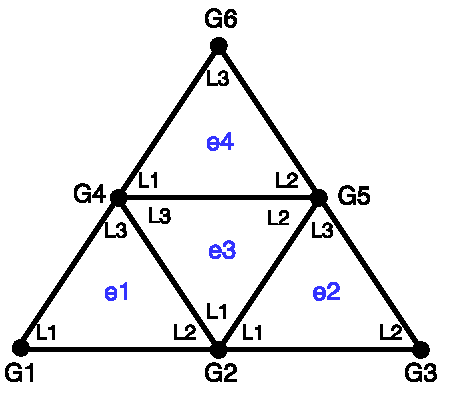
\includegraphics[scale=1]{figuras/id.pdf}
	\caption{Identificadores de elementos e nós}
	\label{fig:numeracao}
\end{figure}

\subsection{Seleção das funções de interpolação}
\label{sec:interp}
O passo seguinte é a escolha das funções de interpolação (ou função de base ou de forma) \cite{huebner} que fornece uma aproximação da equação original dentro de cada subdomínio \cite{jin}. 
A função interpoladora escolhida geralmente é um polinômio, e isso ocorre por dois motivos a priori \cite{desai}:

\begin{itemize}  
	\item Facilidade de manipulação matemática, principalmente derivação e integração;
	\item Aproximação satisfatória quando truncado em uma ordem qualquer.
\end{itemize}

Na prática são escolhidos polinômios de primeira ou segunda ordem, mas ordens superiores podem ser adotadas para reduzir o erro de aproximação, sobretudo em bordas com curvaturas, no entanto, ocorre também o aumento da carga computacional \cite{jin}.

Seja a função $\phi$ desconhecida, da qual se deseja obter uma aproximação. A nível elementar, a função $\tilde{\phi^e}$ aproxima $\phi$ dentro do domínio do elemento $e$. O valor $\tilde{\phi^{e}_i}$  é a aproximação do valor de $\phi$ sobre o nó $i$ de $e$. Considerando um subdomínio bidimensional triangular, o valor aproximado em cada nó de um elemento é dado pela equação \ref{eq:interp}.

\begin{equation}
\label{eq:interp}
\tilde{\phi^e_i} = a^e + b^e x^e_i + c^e y^e_i
\end{equation}

Desta forma, a função que aproxima os valores dentro de todo o domínio $e$ é pode ser dada pela equação \ref{eq:interpol}.

\begin{equation}
\label{eq:interpol}
\tilde{\phi^e} = \sum_{j=1}^{n}{N_j^e (x, y) \phi_j^e} = 
\{N^e\}^T \{\phi^e\}
\end{equation}

Para manter esta aproximação em conformidade com os valores $\tilde{\phi^e_1}$, $\tilde{\phi^e_e}$ e $\tilde{\phi^e_3}$ em cada nó, a função $N_i^e$ deve ser escolhida de forma que seu comportamento seja o mesmo do delta de Kronecker, como mostra a equação \ref{eq:kron} a seguir.

\begin{equation}
\label{eq:kron}
N_i^e(x^e_j, y^e_j) = \delta_{ij} = \begin{cases}
1, \ i = j\\
0, \ i \neq j
\end{cases}
\end{equation}

As funções de interpolação mais comuns pertencem às famílias de funções Lagrange e Serendipity \cite{zien, volakis}.

\subsection{Formulação do sistema de equações}
Na abordagem variacional destaca-se o método de Ritz, ou Rayleigh-Ritz, o qual tem por objetivo, minimizar o funcional variacional, ou funcional de energia, do problema aproximado \cite{volakis}. Embora tal abordagem tenha sido historicamente utilizada e possua fundamentação física e matemática, sua adoção, em muitos casos, é mais complicada em relação ao Método dos Resíduos Ponderados, pois demanda a formulação variacional do problema. Desta forma, se um problema é dado por um modelo diferencial, é necessário se obter a partir deste modelo a forma variacional equivalente, para só então se aplicar o método para a obtenção do sistema de equações. No eletromagnetismo, a formulação variacional das equações de Maxwell não é bem estabelecida \cite{jin}.

Para problemas que apresentam explicitamente condições de Dirichlet no contorno e cujo operador $\mathcal{L}$ é linear e auto-adjunto, é possível se obter imediatamente o funcional de energia correspondente \cite{zien}, no entanto, como mostra \cite[p. 29]{volakis}, para este tipo de operador a mesma integral da formulação variacional é obtida pelo método de Galerkin.


Seja a equação \ref{eq:operador}, uma equação de um PVC na qual $\mathcal{L}$ é um operador diferencial, $f$ é uma função de excitação conhecida e $\phi$ é a solução procurada.

\begin{equation}
\label{eq:operador}
\mathcal{L} \phi = f
\end{equation}

Se substituirmos a solução exata pela sua aproximação apresentada na equação \ref{eq:interpol}, um resíduo $r$ surge, como pode ser visto na equação \ref{eq:residuos}, em decorrencia dos erros de aproximação.

\begin{equation}
\label{eq:residuos}
r = \mathcal{L} \tilde{\phi} - f \neq 0
\end{equation}

Embora o resíduo em cada elemento seja diferente de zero em sua maioria, deseja-se que o resíduo total seja igual a zero. Para que isso seja possível, uma função de poderação $w_i$ é introduzida para cada subdomínio $e$. Desta forma na média dos $M$ subdomínios de $\Omega$ a condição residual é atendida \cite{volakis}.
As equações \ref{eq:res1} e \ref{eq:res2} correspondem ao sistema de resíduos ponderados. A ideia chave dessa abordagem é transformar o problema de valor de contorno para um sistema linear que forneça o valor aproximado. 

\begin{equation}
\label{eq:res1}
R_i^e = \int_{\Omega}{w_i^e r \ d\Omega} = 0 \qquad i = 1,2,3.
\end{equation}

\begin{equation}
\label{eq:res2}
R_i^e = \int_{\Omega}{w_i^e [\mathcal{L} \tilde{\phi} - f] \ d\Omega} = 0
\end{equation}  


A escolha particular de $w_i^e = N^e_i$ configura o método de Galerkin, o qual, para um operador $\mathcal{L}$ auto adjunto a matriz do sistema é simétrica e equivalente à matriz gerada pelo método de Ritz. Após a substituição da equação \ref{eq:interpol} em \ref{eq:res2} obtem-se a equação \ref{eq:galerkin}, a qual forma um sistema esparso de equações lineares como o apresentado em \ref{eq:sistema}.


\begin{equation}
\label{eq:galerkin}
R_i^e = \int_{\Omega}{N_i^e \mathcal{L} \{N\}^T \{\phi\} \ d\Omega\}} - \int_{\Omega}{N^e_i f \ d \Omega} = 0
\end{equation} 


\begin{equation}
\label{eq:sistema}
[K]\{\phi\} = {b}
\end{equation}  

É importante colocar que o parâmetro $w_i$ deve ser um conjunto de funções integraveis, linearmente independentes
\cite[p. 60]{reddy}. Alguns casos especiais do método dos resíduos ponderados são obtidos a partir da escolha de $w_i$:

\begin{equation}
\label{eq:metPond}
\begin{tabular}{ l l }
Método de Petrov-Galerkin & $ w_i = \psi_i \neq \phi_i $ \\ 
Método de Galerkin & $ w_i = \phi_i $\\  
Método dos Mínimos quadrados & $ w_i = \frac{d}{dx} \left(a(x)\frac{d \phi_i}{dx}\right) $ \\ 
Método da colocação & $ \delta(x - x_i)  $ 
\end{tabular}
\end{equation}

\subsection{Método dos elementos finitos em 2 dimensões}
\label{sec:fem2d}

\chapter{Desenvolvimento}

O desenvolvimento deste trabalho está  dividido nas etapas de \textit{validação do problema} e \textit{aplicação das estratégias}. Na primeira são apresentados os recursos utilizados para modelar o problema e para definir as possíveis estratégias de solução. De posse das informações obtidas nesta etapa, são definidos na etapa seguinte os métodos e as estruturas de dados adotados em cada linguagem de programação e arquitetura de processamento.

\section{Materiais e métodos}
O ambiente de desenvolvimento MATLAB\textsuperscript{\textregistered} foi adotado para a realização da etapa de validação do problema. A motivação dessa escolha se deu pela facilidade da manipulação de matrizes oferecida pelo ambiente e pela existência de ferramentas dedicadas à especificação de PVCs e à programação paralela.
A aplicação das estratégias propostas na etapa de validação nas linguagens e arquiteturas adotadas neste trabalho é feita pela adequação da sintaxe e do paradigma de programação da implementação realizada no MATLAB\textsuperscript{\textregistered}. 

\subsection{Especificação da geometria}
O problema \textit{benchmark} utilizado neste trabalho é o exemplo $10.3$ do livro Análise de Circuitos de \citeonline{boylestad2011} e é ilustrado na figura \ref{fig:placas}. O capacitor é composto de duas placas quadradas paralelas com lado de $2$ polegadas, cuja distância entre elas é de $\frac{1}{32}$ polegadas. O problema informa que a diferença de potencial entre as placas é de $48V$, dessa forma foi assumido que uma das placas possui $48V$ e e que a outra está aterrada.

\begin{figure}[!htb]
	\centering
	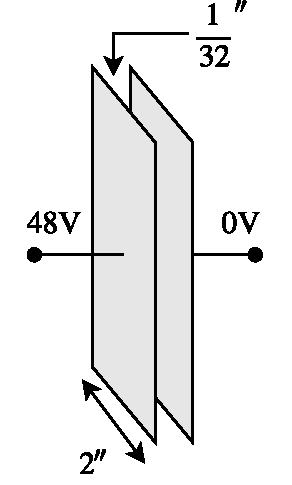
\includegraphics[scale=0.9]{figuras/placas.pdf}
	\caption{Capacitor de placas paralelas}
	\label{fig:placas}
\end{figure}

A fim de se realizar uma análise mais ampla do problema a distribuição do campo elétrico será calculada entre as placas mas também no espaço ao redor. Será considerada uma região quadrada de $16cm$ de lado como mostra o esquema na figura \ref{fig:mesh}{(a)}. Também foi considerado que a espessura de cada placa é a metade da largura da região entre elas, ou seja, $\frac{1}{64}$ polegadas.


A fim de se obter um parâmetro da corretude dos resultados obtidos neste trabalho, foi feita a simulação do problema na \textit{partial differential equation toolbox} do MATLAB\textsuperscript{\textregistered}. Por meio dessa ferramenta é possível programaticamente e via interface gráfica definir a equação diferencial que rege o problema, a geometria, as condições de contorno, a malha inicial e seus refinamentos bem como a solução e exibição dos resultados do PVC. As figuras \ref{fig:mesh}{(b)} e \ref{fig:mesh}{(c)} mostram a geometria e a malha inicial modeladas com o auxílio da interface gráfica da \textit{pdetool}.

\subsection{Obtenção dos valores de referência}


\begin{figure}%
	\centering
	\subfloat[Esquema da região de análise]{{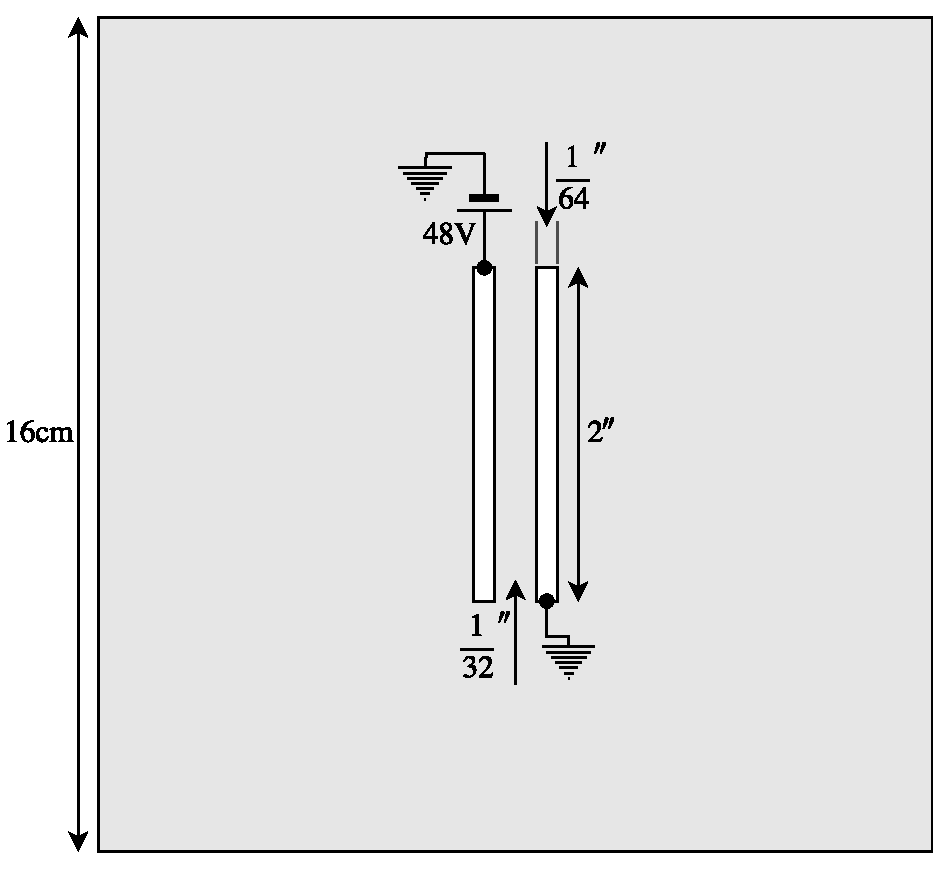
\includegraphics[scale=0.5]{figuras/espaco.pdf} }}%
	\qquad	
	\subfloat[Região de análise com malha]{{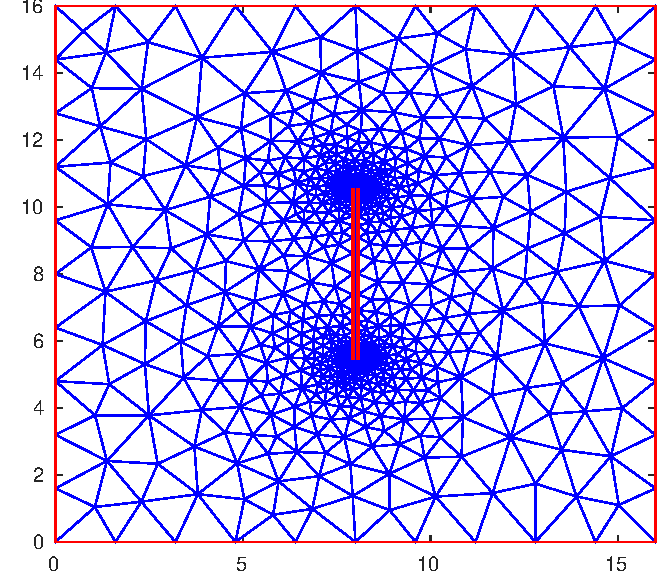
\includegraphics[scale=0.4]{figuras/mesh.pdf} }}%
	\qquad
	\subfloat[Zoom sobre as placas do capacitor]{{\includegraphics[scale=0.4]{figuras/mesh_zoom.pdf} }}%
	\caption{Geometria do capacitor de placas paralelas}%
	\label{fig:mesh}%
\end{figure}

Definidas a geometria e a malha, foram feitas as atribuições das condições de contorno de Dirichlet nas $4$ bordas da seção de cada placa. À placa da esquerda foram atribuídos $48V$ e $0V$ para a placa da direita. Para se definir a EDP do problema é necessário atribuir valores aos coeficientes da fórmula geral de EDPs elípticas, mostrada na equação \ref{eq:geral}.



\begin{equation}
\label{eq:geral}
- \bigtriangledown\cdot(c\bigtriangledown(u)) + au = f
\end{equation} 

Na equação de Laplace, que modela a distribuição do potencial elétrico, apenas o coeficiente $c$ é diferente de zero. A constante $c$ corresponde à permissividade no vácuo na equação de Poisson, mas como a densidade volumétrica de carga representada por $f$  e o auto valor $a$ são iguais a zero na equação de Laplace, $c$ passa a valer $1$. Estabelecidos os valores das constantes a solução do problema pode ser obtida, como mostram as figuras \ref{fig:solPde}{(a)} e \ref{fig:solPde}{(b)}.

\begin{figure}%
	\centering	
	\subfloat[Distribuição do potencial em Volts e fluxo do campo elétrico em Volts/centímetro (vetores normalizados)]{{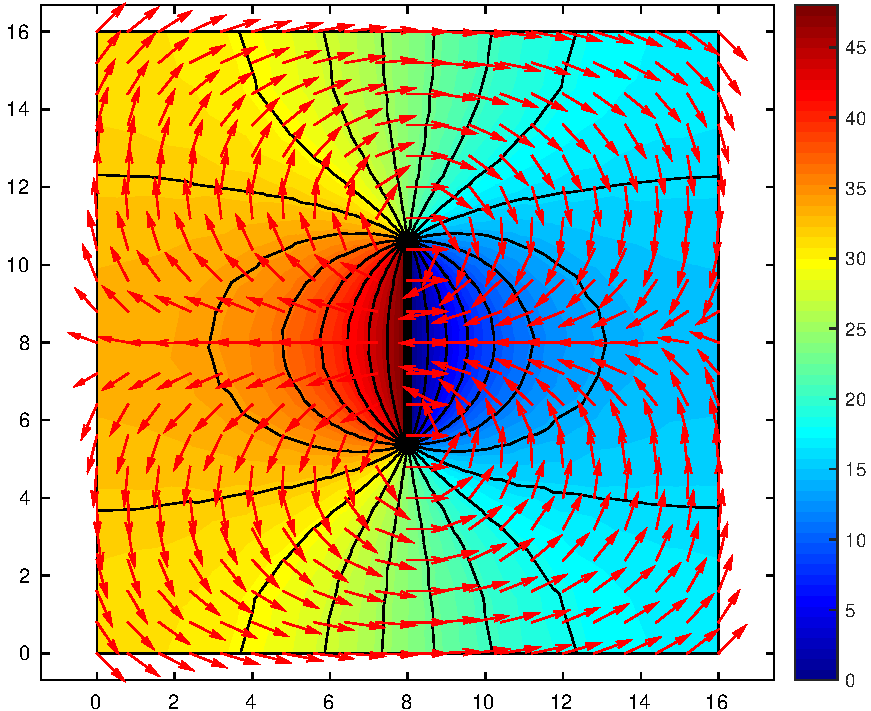
\includegraphics[scale=0.4]{figuras/potcampo.pdf} }}%
	\qquad
	\subfloat[Distribuição do potencial entre as placas]{{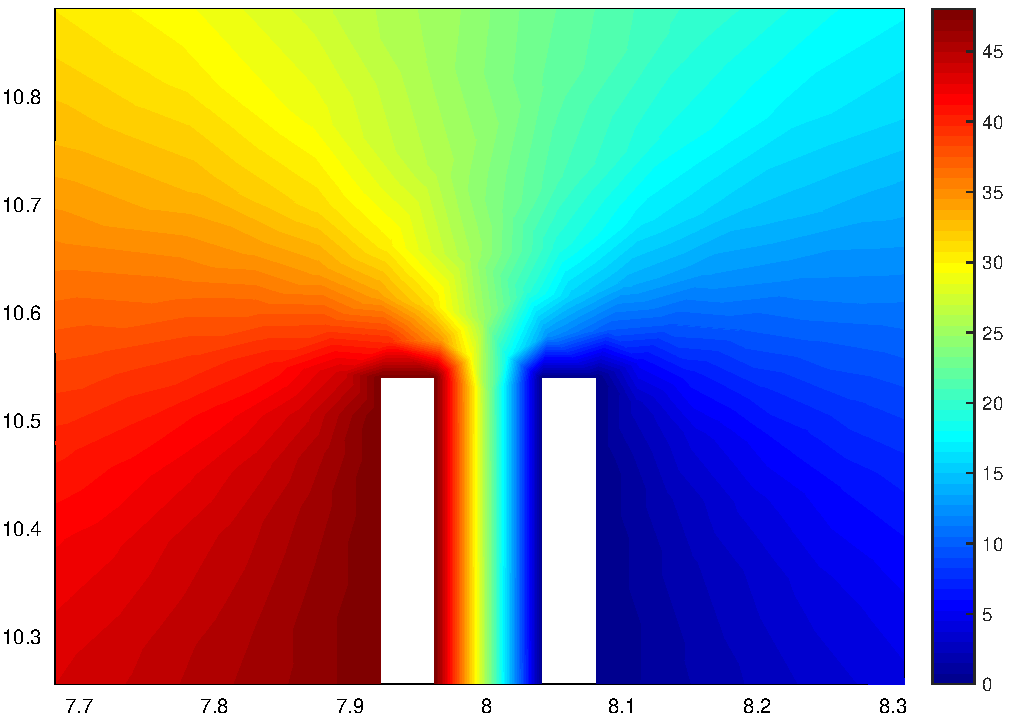
\includegraphics[scale=0.4]{figuras/potzoom.pdf} }}%
	\qquad
	\subfloat[Pontos de referência do potencial elétrico]{{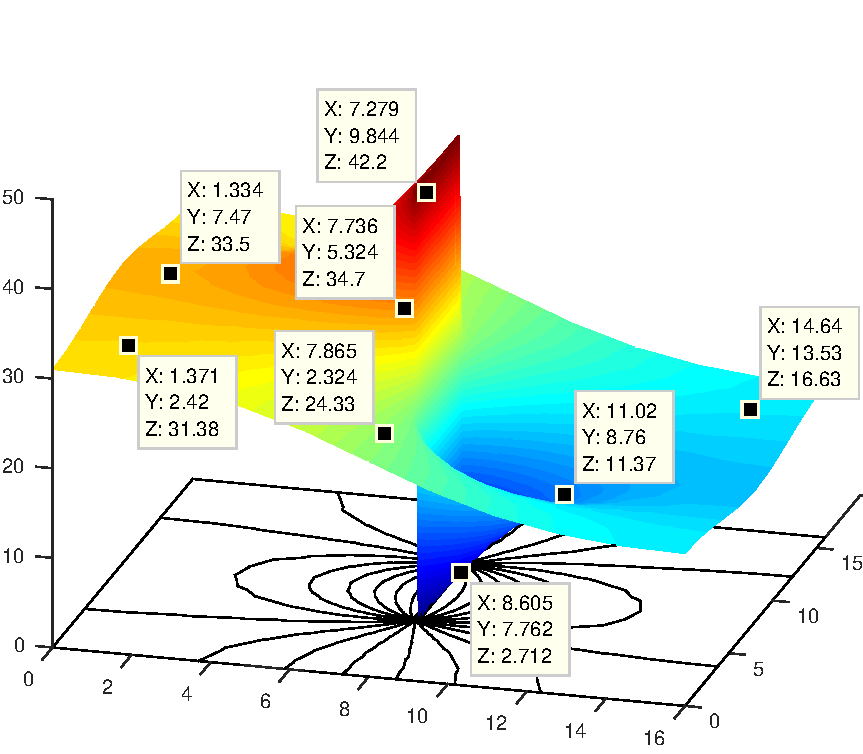
\includegraphics[scale=0.4]{figuras/valpot2.pdf} }}%
	\qquad
	\subfloat[Pontos de referência do campo elétrico]{{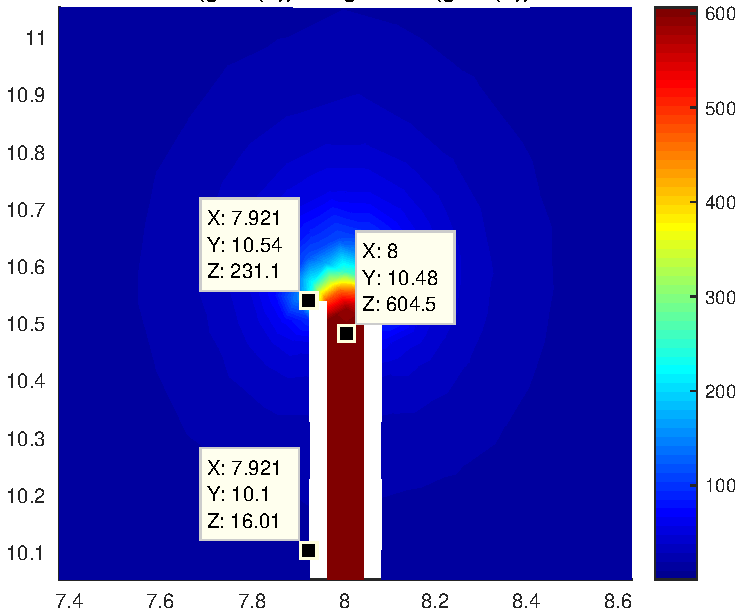
\includegraphics[scale=0.4]{figuras/valCampo.pdf} }}%
	\caption{Solução do PVC com a \textit{pdetool}}%
	\label{fig:solPde}%
\end{figure}

De posse da solução da \textit{pdetool}, foram tomados $8$ pontos de referência da distribuição do potencial e $3$ pontos de referência do campo elétrico. A localização e os valores destes pontos são apresentados na figuras \ref{fig:solPde}{(c)} e \ref{fig:solPde}{(d)}.

\subsection{Implementação do FEM}
Após a simulação e obtenção dos valores de referência foi realizada a implementação do método dos elementos finitos em duas dimensões, conforme o apresentado na seção \ref{sec:fem2d} do referencial teórico.
A fim de não tirar proveito das funções do MATLAB\textsuperscript{\textregistered} de forma a manter a generalidade da solução implementada e a facilidade de transcrevê-la para outras linguagens, foram utilizadas nos algoritmos deste trabalho apenas as funções da \textit{PDE toolbox} relativas à geometria, geração da malha e exibição dos resultados. No pseudocódigo \ref{alg:FEM} as palavras destacadas em itálico são variáveis, as funções destacadas em negrito fazem parte do MATLAB\textsuperscript{\textregistered} e as funções descritas nas linhas de $9$ a $12$ são detalhadas no exemplo da seção \ref{sec:fem2d}. A tabela \ref{tab:matlabFun} contém a descrição das funções utilizadas.


\begin{table}[!ht]   
	\centering
	\begin{tabular}{|l|p{10cm}|}  
		\hline
		\textbf{Função} 
		& \textbf{Descrição} 
		\\  
		\hline
		\textbf{load} 
		& Carrega para o \textit{workspace} as variáveis salvas nos arquivos \textit{.mat}. 
		\\
		\hline
		\textbf{decsg}  
		& Cria a geometria do problema por meio da associação de regiões primitivas. O espaço de análise do capacitor de placas paralelas, por exemplo é composto por $2$ retângulos e $1$ quadrado.
		\\
		\hline		
		\textbf{createpde} 
		& Instancia um modelo de PDE contendo $n$ equações.
		\\
		\hline		 
		\textbf{geometryFromEdges} 
		& Vincula a geometria originada da função $decsg$ ao modelo de PDE gerado por $createpde$.
		\\
		\hline		
		\textbf{generateMesh} 
		& Cria uma malha sobre a geometria do modelo de PDE. Parâmetros adicionais podem ser incluídos para modificar a qualidade malha ou a ordem dos elementos (ver \ref{sec:interp}). O parâmetro $Hmax$ determina o tamanho máximo das arestas dos elementos.
		\\
		\hline		 
		\textbf{meshToPet} 
		& Obtém as matrizes de pontos, arestas e triângulos, as quais serão utilizadas na geração das matrizes elementares e da matriz global.
		\\
		\hline	
		geraMatElementares
		& À partir dos dados da triangulação da malha, gera a matriz de cada elemento por meio das funções de aproximação e interpolação.
		\\
		\hline
		geraMatGlobal
		& Realiza a agregação ou o mapeamento das matrizes elementares no sistema global. A matriz resultante é esparsa e sua ordem corresponde ao número de nós da malha.
		\\
		\hline
		atribuiContorno  
		& Atribui os $m$ valores de contorno pré-estabelecidos e com isso realiza a redução dos sistema em $m$ ordens, fazendo com que deixe de ser homogêneo.
		\\
		\hline
		resolveSistLinear
		& Ponto da principal contribuição deste trabalho e consiste na aplicação de métodos numéricos para a solução eficiente de sistemas lineares esparsos.
		\\
		\hline		 
		\textbf{pdePlot}  
		& Função utilizada para a exibição da malha e dos resultados. Conforme os parâmetros adicionais, são plotados gráficos tridimensionais, campos vetoriais e linhas de campo.
		\\
		\hline	
	\end{tabular}
	\caption{Descrição das funções utilizadas no algoritmo do FEM}
	\label{tab:matlabFun}
\end{table}
 
\begin{algorithm}	
	\caption{\label{alg:FEM}Pseudocódigo do FEM} 
	\begin{algorithmic}[1]
		\State{\textbf{load}($dadosGeometria$);}
		\State{\textbf{load}($coordReferencia$);}
		\State{\textbf{load}($dadosContorno$);}
		\State{$g$ = \textbf{decsg}($dadosGeometria$);}
		\State{$m$ = \textbf{createpde}(1);}
		\State{\textbf{geometryFromEdges}($m$,$g$);}
		\State{\textbf{generateMesh}($m$, 'Hmax',$valHmax$);}
		\State{[$p$,$e$,$t$] = \textbf{meshToPet}($m.Mesh$);}
		\State{$C$ = geraMatElementares($p$, $t$);}
		\State{$G$ = geraMatGlobal($C$, $t$);}
		\State{[$A$, $b$] = atribuiContorno($G$, $dadosContorno$);}
		\State{$sol$ = resolveSistLinear($A$,$b$);}
		\State{\textbf{pdeplot}($m$,...);}
	\end{algorithmic}
\end{algorithm}



\subsection{Aplicação das estratégias}

\section{Resultados preliminares}










% ----------------------------------------------------------
% ELEMENTOS PÓS-TEXTUAIS
% ----------------------------------------------------------
\postextual
% ----------------------------------------------------------

% ----------------------------------------------------------
% Referências bibliográficas
% ----------------------------------------------------------
\bibliography{abntex2-modelo-references}
%\bibliography{bibfile}

% ---
% Inicia os apêndices
% ---
\iffalse
\begin{apendicesenv}
\label{chap:apendices}

% Imprime uma página indicando o início dos apêndices
\partapendices

% ---
\chapter{Tabelas do primeiro teste}
apendice

% ---


\end{apendicesenv}
% ---
\fi
\end{document}
